\chapter{Simulating a Time Delay attack}



\section{Scenarios}

For the experimental part of my thesis, a number of attack scenarios will be required. The aim is to investigate various attack vectors which might be used by a sophisticated man-on-the-side threat actor in order to execute an attack while staying undetected. 

\subsection{Background} 

A number of assumptions is stated, in order to narrow the scope of the thesis.

\subsubsection{Attacker policy assumptions}
A sophisticated threat actor would most likely want to avoid detection by anyone protecting the targeted infrastructure.
Therefore, executing an attack which may be detected should be avoided at all costs.
As a consequence, any decisions related to actually executing the attack should be as a result of promising results following a stealthiness assessment process\footnote{Simulations of possible effects could be part of a stealthyness assessment process}. 

\subsubsection{Attack Prerequisites}
A stealthy attack with small impact is preferred over an attack having more severe impacts, at a higher risk of detection.
The ideal attack would be an attack having maximal impact on the target, while the risk of detection being minimal. 


\subsubsection{Attack design challenges}
A part of the challenge would be to design an attack producing a high impact on the target, while staying undetected.

\subsubsection{selected approach}
One possible solution could be to determine the minimal efforts needed in order to execute an attack with a high probability of producing the effects desired, while keeping the attack detection probability low.



\subsection{Definition of scenarios}
In order to provide experimental results in order to answer the Research Questions stated, a number of attack scenarios are defined.

The main method of simulation would be a delayed forwarding of values, where a specified delay $d$ is applied to the PMU input, replacing any sample with sample $s(i)$ with the sample value $s(i-d)$, simulating clock drift, producing effects similar to a \acrlong{tda}.

The simulation could be performed using a number of delay functions, for instancs:
\begin{itemize}
   
\item  \textbf{Exposing the targeted PMU to a constant delay from a specified initiation time} 
    The delay is unaltered from the time of initiation, until the duration of the simulation. 
\item     \textbf{Exposing the targeted PMU to a constant delay for a limited time, from a specified initiation time} 
\end{itemize}
    


\subsection{Attack Implementation}
%The attacks would be implemented as MATLAB functions executing attacks on targets implemented as SIMULINK simulations. The various scenarios would  be required to be sufficiently similar to be implemented as variations of a single attack framework, in order to avoid the need of creating more than a single attack framework.     

%In order to prepare for attacks, a plan might be to implement the techniques described in \cite{gilad2014off}.



\textbf{\cite{barreto2016undetectable} proves the requirement of exposing more than two PMUs to a delay attack, for the attack to be undetectable.}




A number of physical investigations related to the effects of any intended attacks on the intended targets, would increase the knowledge of a potentially complex target, increasing the probability of staying undetected during the attack. In order to avoid exposing expensive and critical power system infrastructure to physical damage or downtime,\footnote{In a test lab environment, downtime could be acceptable, whereas the risk of physical damage of typically expensive equipment may be too high, at least not in the initial phases of investigations.} such practical investigations would preferably be performed in a simulation environment.

\section{Creating a Simulation environment}

This approach could be taken by a threat actor during a phase of investigations in the preparation of the actual attack, for the purpose of learning more about the possible consequences of performing intended actions on the intended target. One of the most important priorities of the threat actor, is to stay undetected for as long as possible. Simulations are designed in order to investigate the selected attack scenarios. The planned attack is implemented using a combination of Simulink and MATLAB. The execution of each simulation will produce corresponding graphs, illustrating any visible effects the attack may have on the system, by analytically comparing the output produced by the attack, with the alternative output of the unmodified, and correct Synchrophasor signal corresponding to  a situation of no attack being performed.

\section{Modelling a PMU}

As the plan of the threat actor is to expose  a number of \acrshort{pmu}s to a time  delay attack, the plan is to build a model of a \acrshort{pmu}, allowing the model to be run while altering any time stamp values required, in order to investigate any observable effects on the output from the \acrshort{pmu}.
 \begin{figure}[ht]
\centering
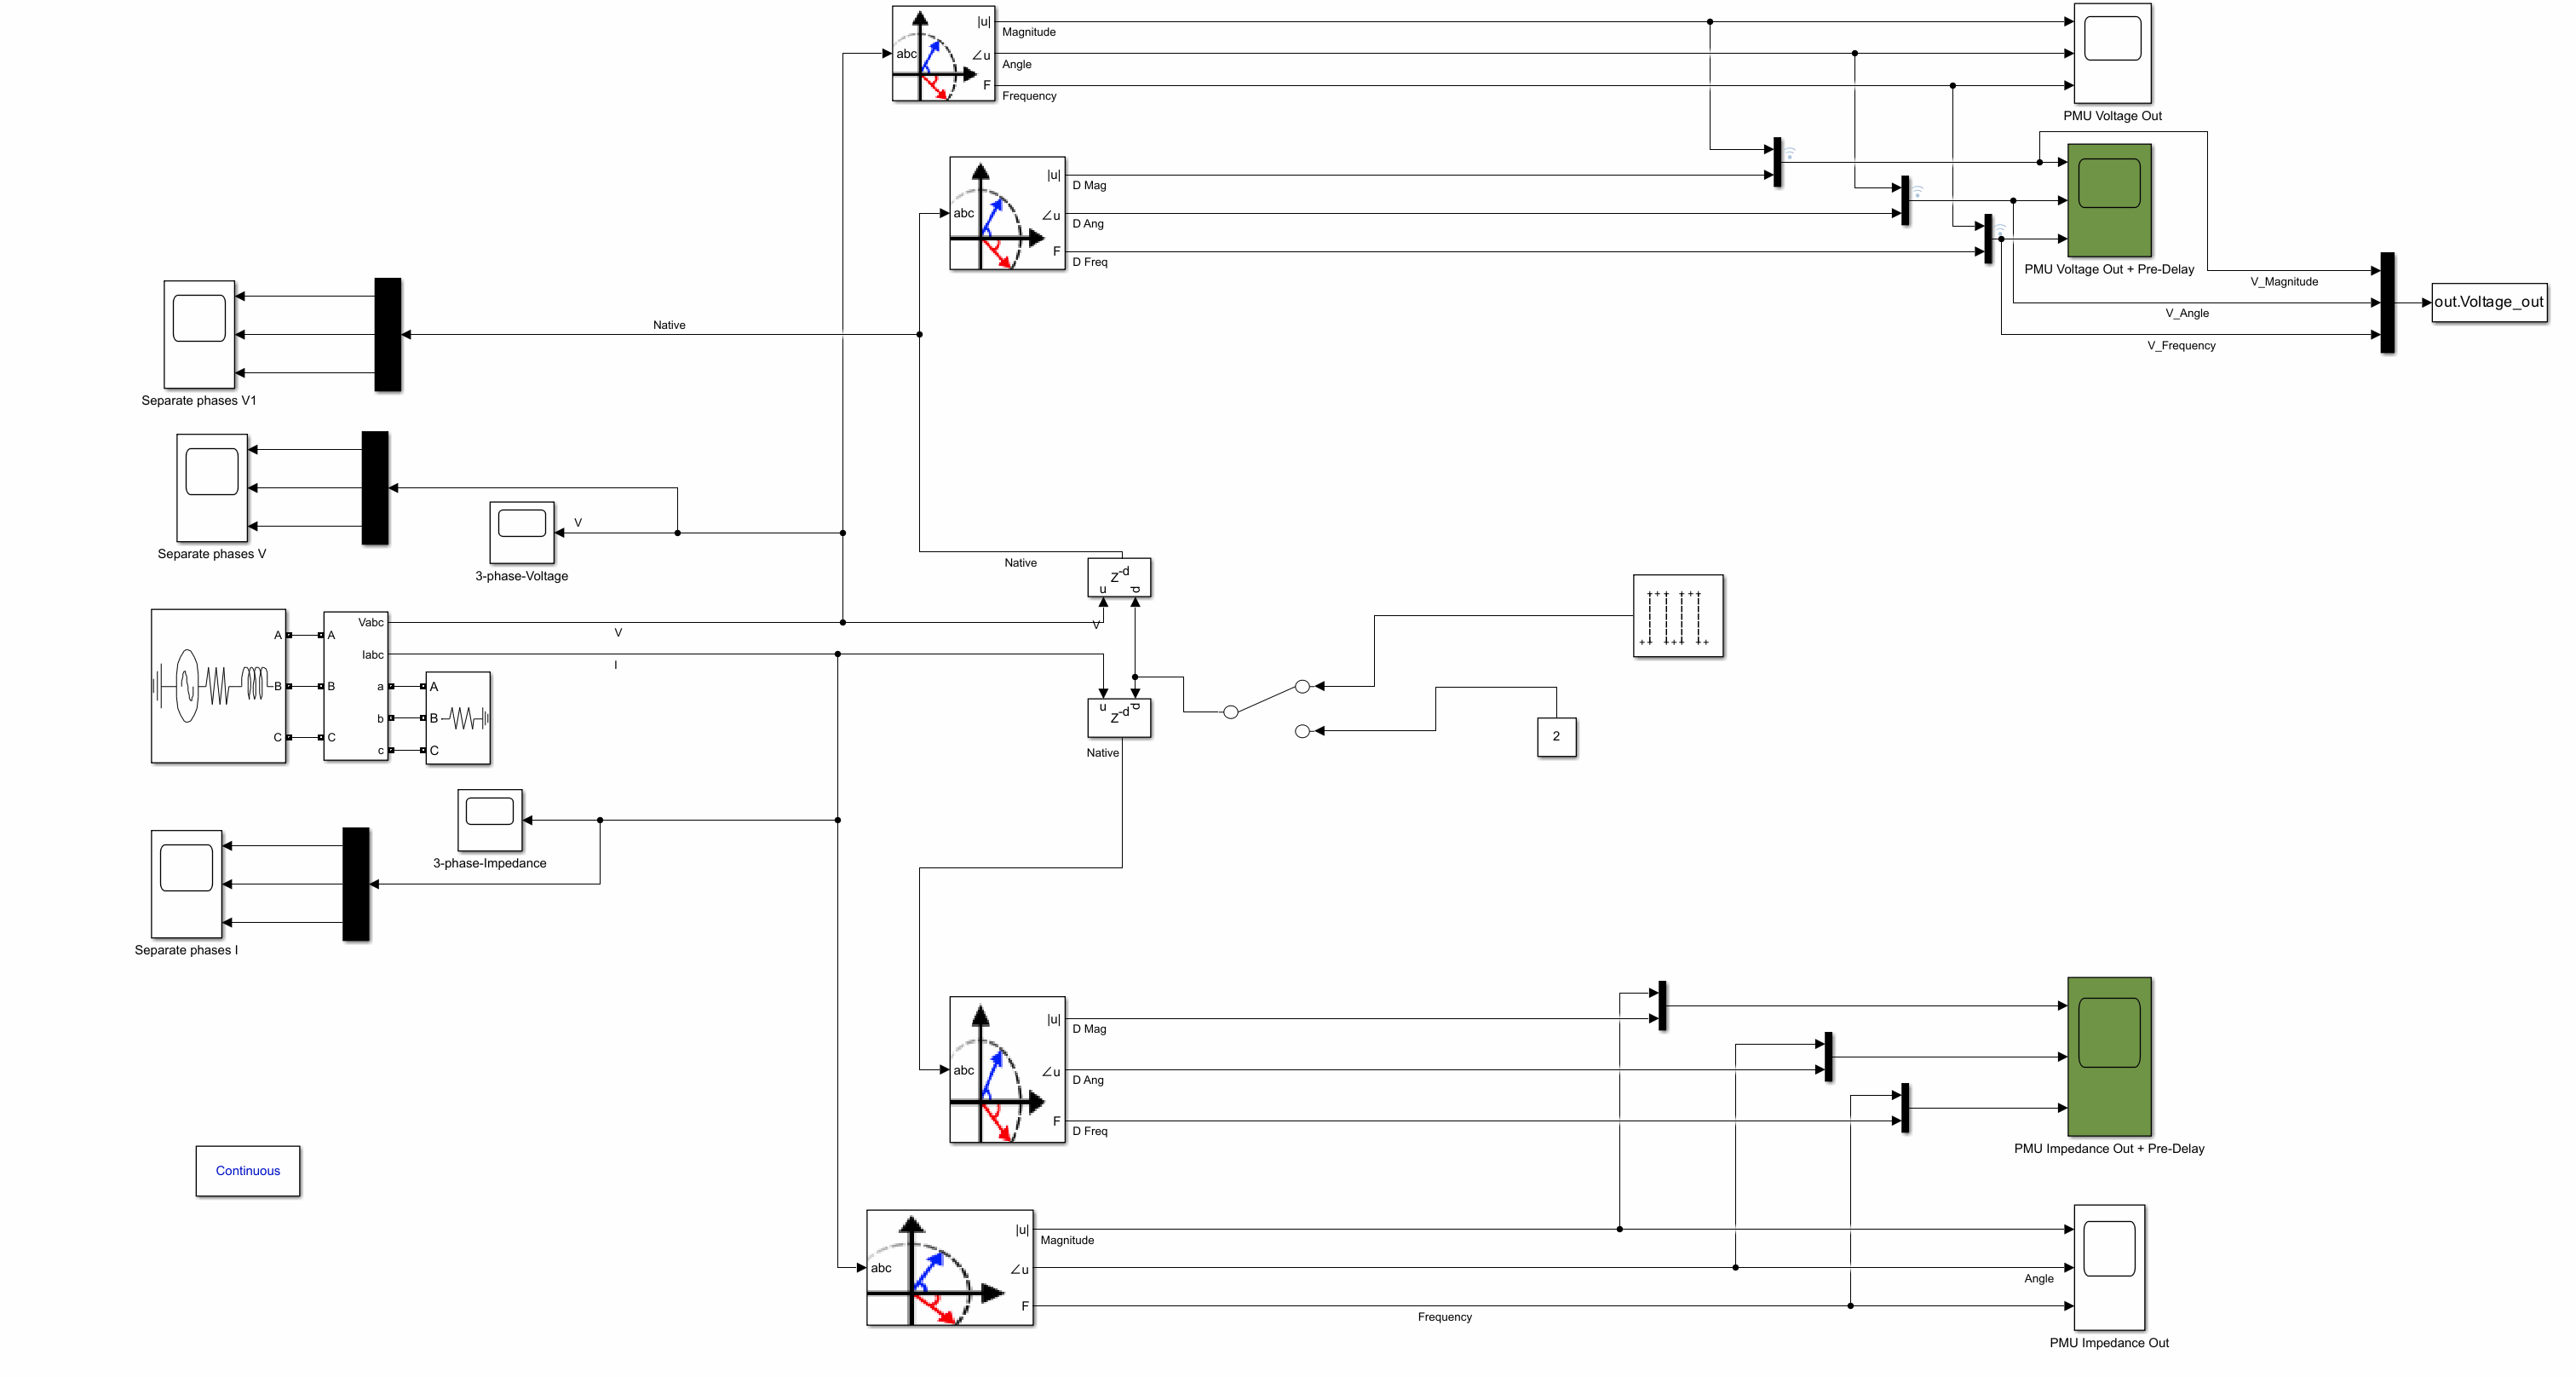
\includegraphics[width=\textwidth]{figures/SimPMU.png}
\caption[PmuSIM SIMULINK model]{A SIMULINK model for the simulation of PMU time delay attacks}

\end{figure}